\section{Conclusioni}
\begin{figure}[H]
	\centering
	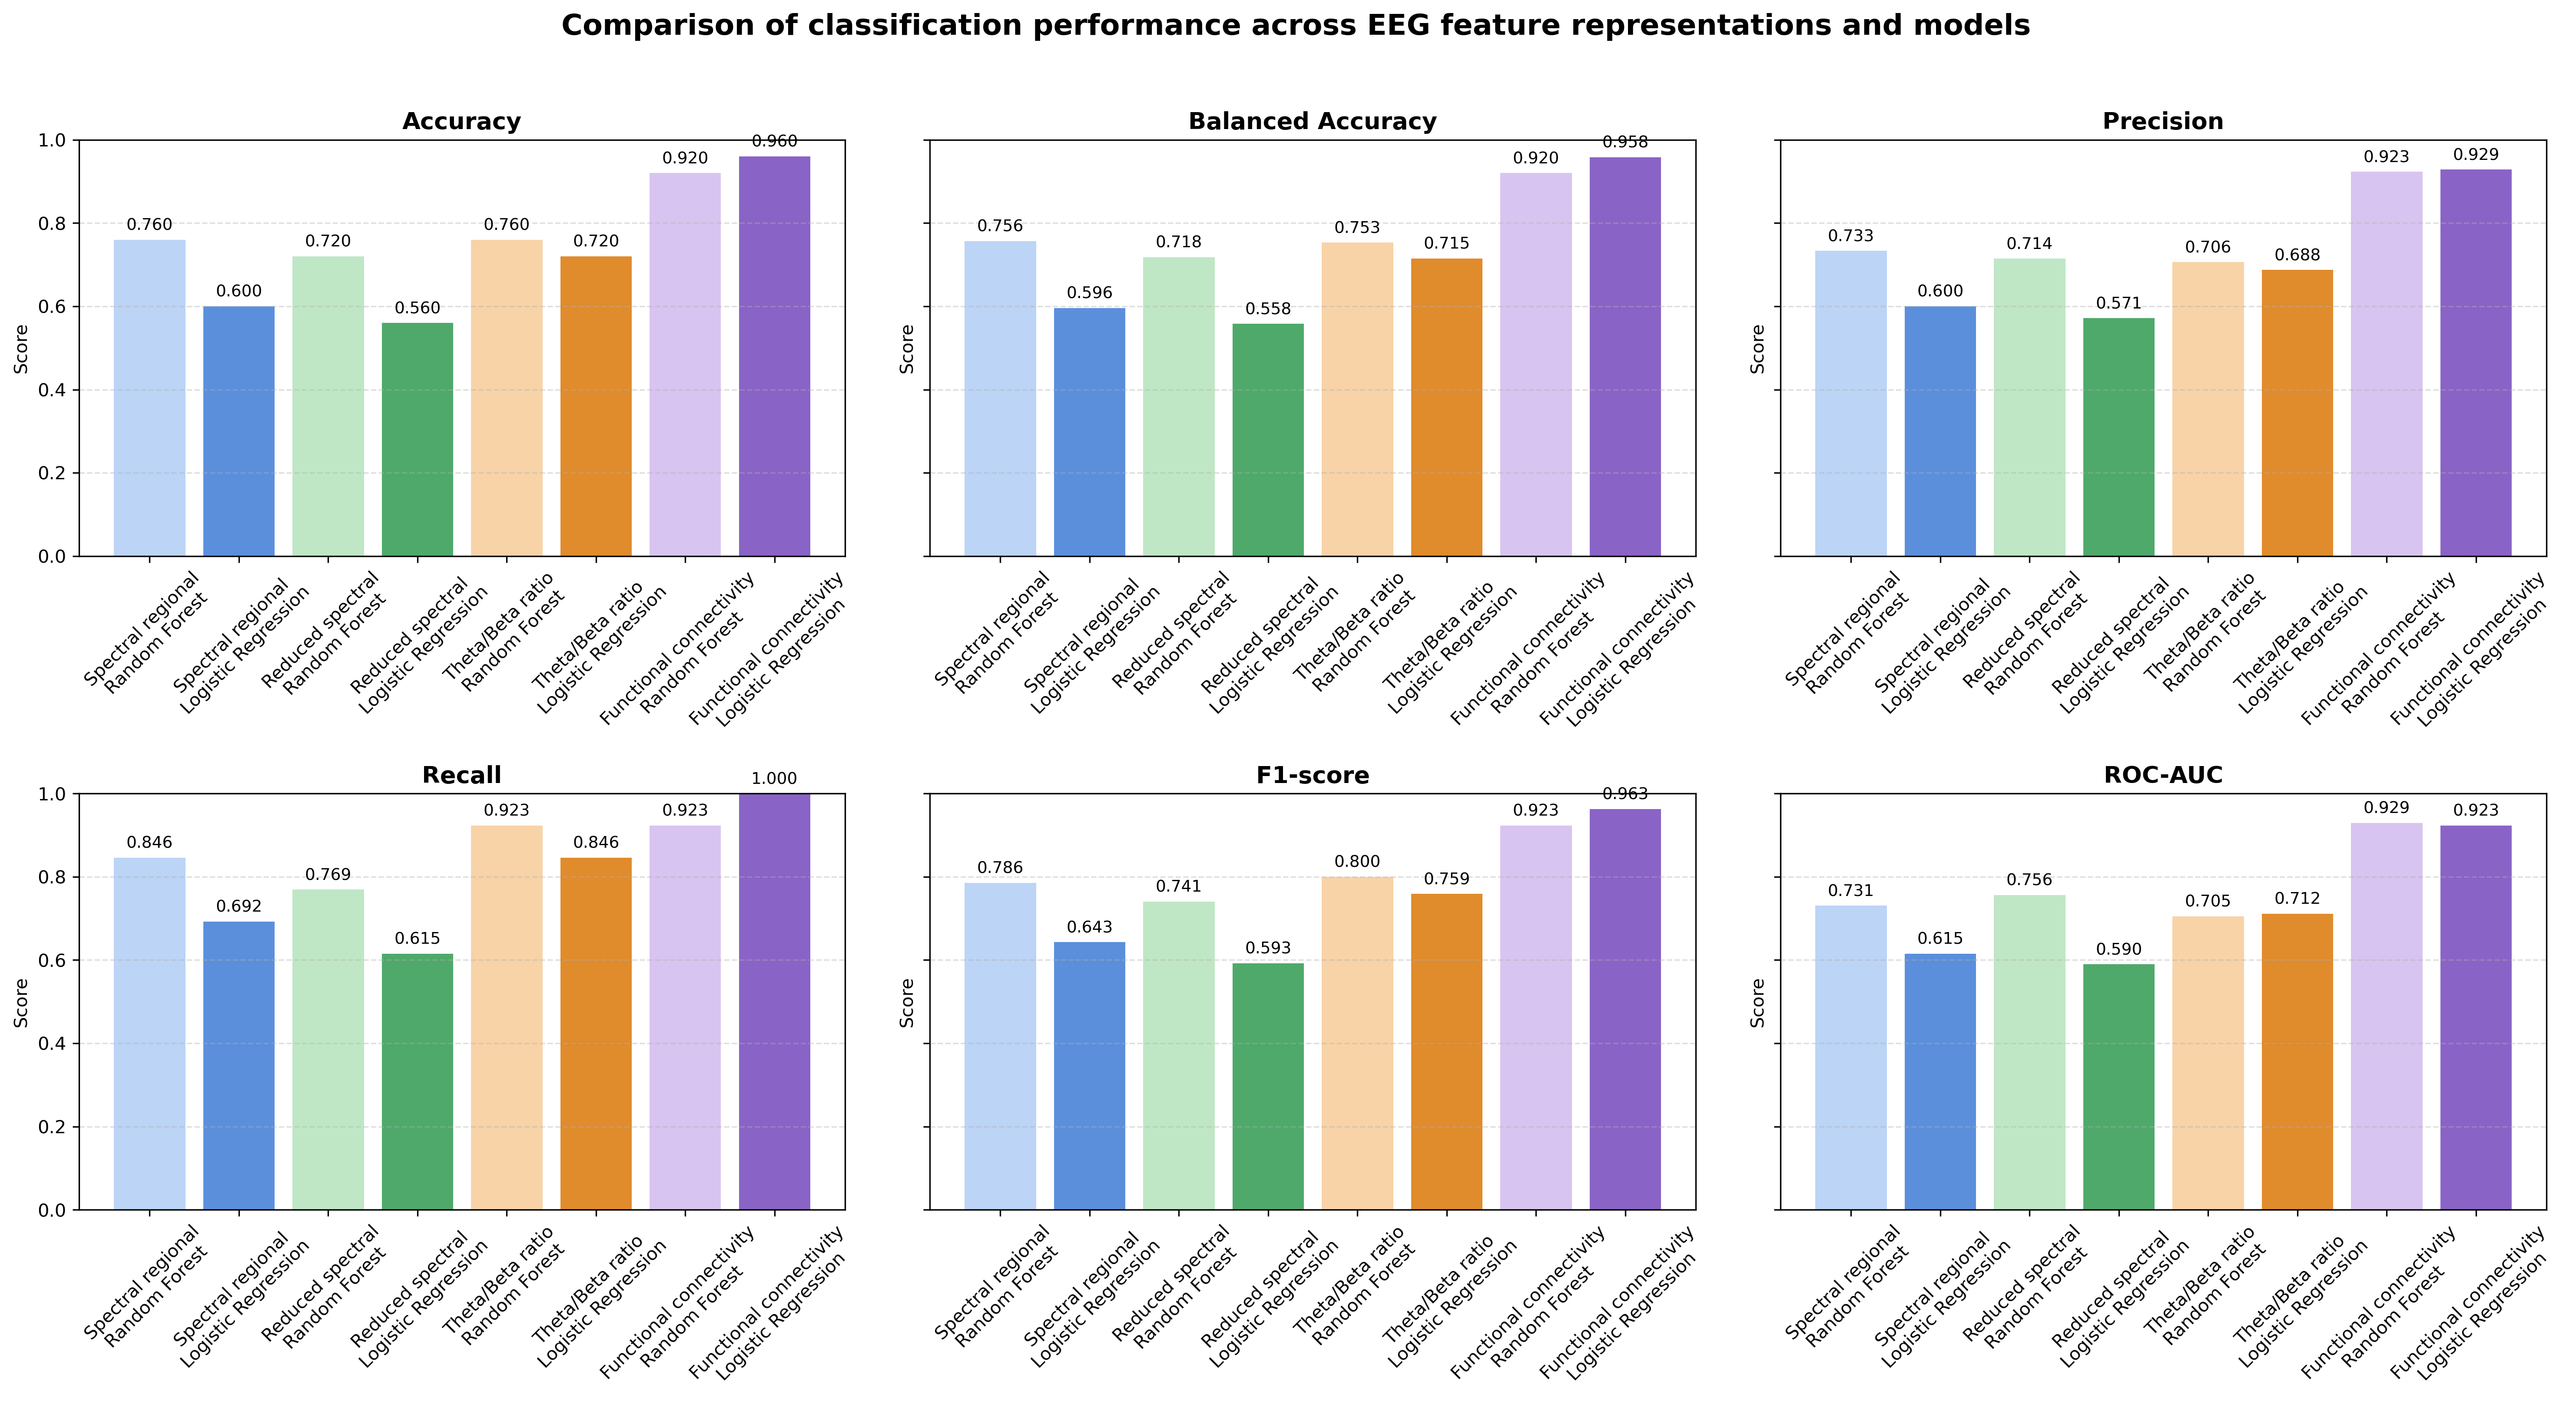
\includegraphics[width=0.98\textwidth]{../figures/5_model_comparison_all_metrics.png}
	\caption{Confronto complessivo delle metriche di classificazione sul test set indipendente per le diverse rappresentazioni EEG e i diversi modelli.}
	\label{fig:overall_model_comparison}
\end{figure}
Il confronto complessivo mostra che le feature di functional connectivity regionale ottengono le prestazioni migliori tra tutte le rappresentazioni EEG considerate. Le feature spettrali e il rapporto theta/beta risultano comunque informative, ma mostrano prestazioni inferiori rispetto alla connettività. Questo suggerisce che, nel dataset analizzato, le relazioni funzionali tra regioni EEG rappresentino una descrizione più efficace per la classificazione ADHD vs Control rispetto alle sole misure di potenza spettrale.

È importante sottolineare alcune limitazioni. Il numero di soggetti è relativamente ridotto e il dataset deriva da una specifica condizione sperimentale. 

Sviluppi futuri potrebbero includere il confronto con ulteriori misure di connettività. 